\documentclass{article}

\usepackage{float}
\usepackage{colortbl}
\usepackage{multirow}
\usepackage{subcaption}
\usepackage[font={small,it}]{caption}
\usepackage{wrapfig}
\usepackage{graphicx}
\usepackage{titlesec}
\usepackage{tablefootnote}

\titleformat{\paragraph}
{\normalfont\normalsize\bfseries}{\theparagraph}{1em}{}
\titlespacing*{\paragraph}
{15pt}{3.25ex plus 1ex minus .2ex}{1.5ex plus .2ex}



\graphicspath{ {images/} }

\title{A simple approach to word jumbles}
\author{Damon Barrett \\ 0834104}
\date{\today}

\begin{document}
	\maketitle
	\newpage 
	
	\tableofcontents
	\listoffigures
	\newpage 
	
	\section{Background}
	
	\begin{wrapfigure}{r}{0.33\textwidth}
		\centering
		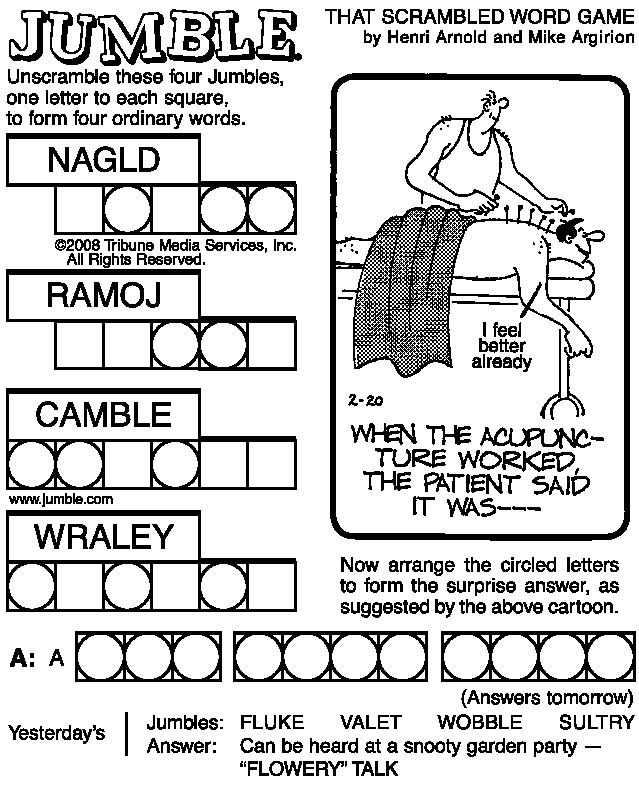
\includegraphics[width=0.33\textwidth]{j1.png}
		\caption{An example of a word jumble.}
	\end{wrapfigure}
	
	A word jumble is a type of word puzzle tasking the user with solving a series of anagrams.  A word jumble consists of a number of \textit{clues}.  Clues are anagrams that must be solved and written into the corresponding \textit{answer (clue) entry}.  An answer entry consist of a series of square boxes, each meant to hold a single letter of the solved anagram.  Select boxes in the answer entry contain circles, these circles designate \textit{key letters}.  Key letters are positionally dependent parts of the solution to the clue anagrams.  Together the key letters extracted from the clue entries form an additional anagram which must be solved to fit the \textit{final answer entry}.  The final answer entry is the bottommost entry on the word jumble. It defines the solved structure of the anagram formed by the key letters.  The final anagram is considered the ultimate goal when solving a word jumble. \par
	The word jumble also contains various text, and a comic positioned as a hint for the final anagram.  However, these are ignored as this method of solving is purely concerned with the clues and entries. \par 
	
	\section{Algorithm}
	The following algorithm assumes that the input image is a binarized, 8-bit word jumble, with a minimum width of 250px.  Images with large amounts of noise, especially around the edges, can present this technique with problems.
	\subsection{Input image cropping}
	The first stage of the algorithm for solving the word jumbles involves cropping unnecessary features out of the image.  Only the clues, the clue entries, and the answer entry are leveraged by the algorithm in solving the word jumble, meaning everything else can be cropped out. Unnecessary features are cropped out of the image because they can cause issues with the clue recognition and particle analysis subprocesses performed later on. \par
	Three crops are performed on the image $C_{title}$, $C_{hint}$, and $C_{ans}$.  $C_{title}$ removes the title text and instructions.  $C_{hint}$ removes the hint comic and associated text.  $C_{ans}$ removes any text below the final answer entry.  Each crop is defined by two opposing corner points framing the area to be removed from the image.
	
	\begin{figure}[h]
		\centering
		\begin{subfigure}{.5\textwidth}
			\centering
			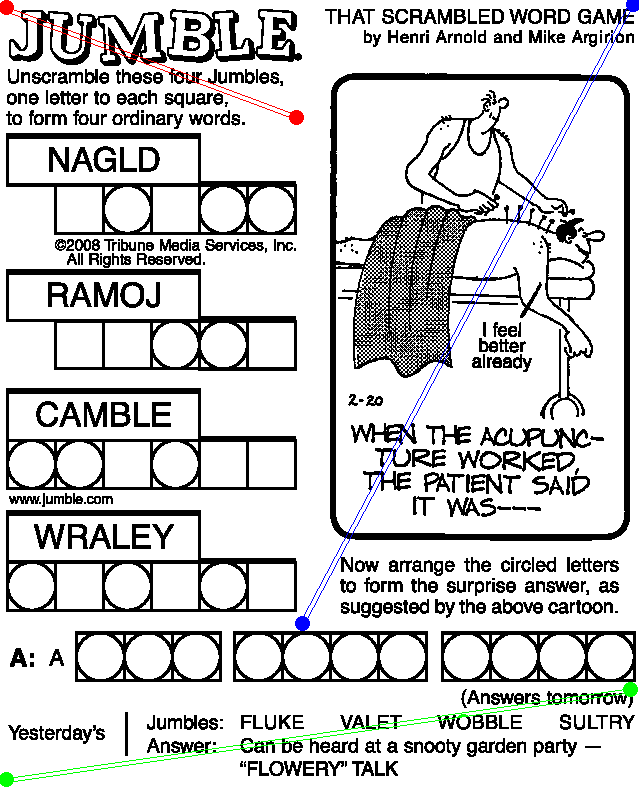
\includegraphics[width=.9\linewidth]{j1_example}
			\caption{The regions to cropped from the jumble.}
			\label{fig:sub1}
		\end{subfigure}%
		\begin{subfigure}{.5\textwidth}
			\centering
			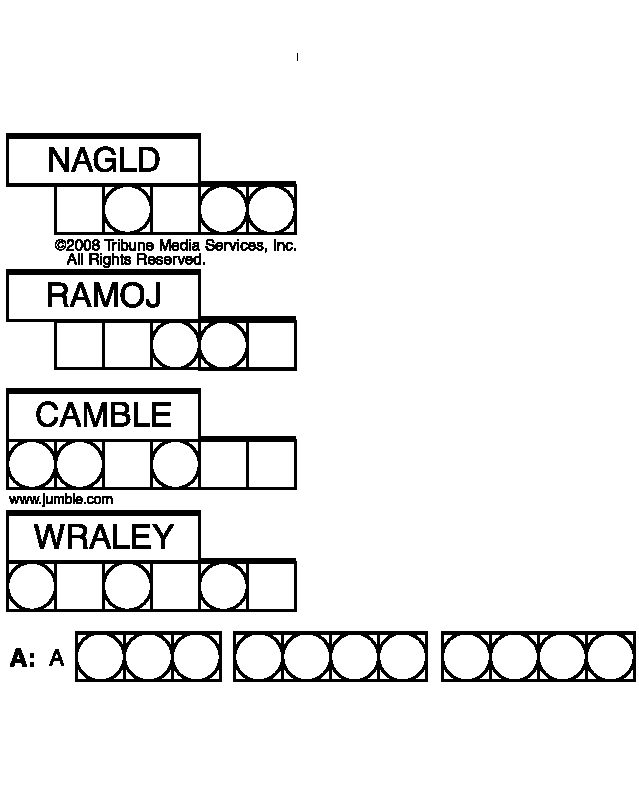
\includegraphics[width=.9\linewidth]{j1_cropped}
			\caption{The resulting image after cropping.}
			\label{fig:sub2}
		\end{subfigure}
		\caption{Cropping a word jumble.}
		\label{fig:test}
	\end{figure}

	\subsubsection{Significant Horizontal Line Detection}
	To locate the points used in cropping the word jumbles, a technique I'm calling Significant Horizontal Line Detection (SHLD) is employed.  SHLD detects horizontal lines in a image that are greater than some significance factor ($\theta$) times the width of the image.  In this case $\theta = 0.1$ is chosen, meaning for a line to be detected by SHLD it must be at least 10\% the width of the image.  \par 
	
	\begin{wrapfigure}{r}{0.4\textwidth}
		\centering
		\fbox{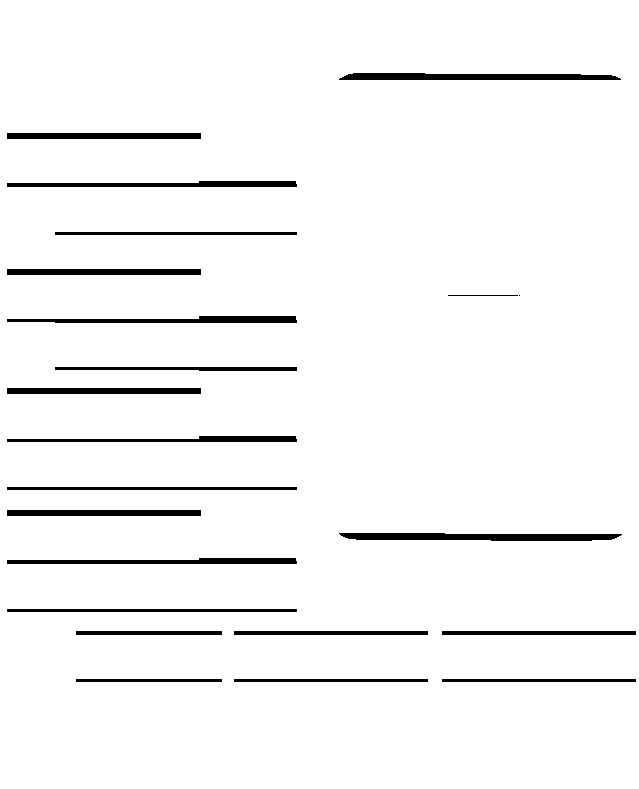
\includegraphics[width=.4\textwidth]{shld}}
		\caption{Lines detected by SHLD (before cropping).}
		\vspace{-20pt}
	\end{wrapfigure}
	
	Performing SHLD on a word jumble produces a set of lines, $L$, found in the image.  $L$ can be easily manipulated to locate positional landmarks within the word jumble.  \par
	
	The first point for $C_{title}$ is located at the origin of the image.  The second point for $C_{title}$ is generated by taking the $x$ value where the clue entries end, and the $y$ value of the first clue.	The first point for $C_{hint}$ is the top right corner of the image.  The crop area for $C_{hint}$ extends to the point defined in the $x$ by the end of the clue entries and in the $y$ by the top of the final answer entry.
	Finally, the first point for $C_{ans}$ is taken as the bottom left corner of the image, with a crop area extending all the way across the image and up to the bottom of the final answer entry.
	
	\subsection{Jumble feature extraction}
	The next step of the algorithm is concerned with extracting features from the jumble that can be provided to the solver.  This step takes the cropped image resulting from the first step as input.   Two separate processes are applied to the cropped image to provide as much information to the solver as possible.  The first subprocess performs particle analysis to determine the composition of each entry in terms of key and regular letters.  The second process extracts the clue strings from the cropped image and uses Optical Character Recognition (OCR) to determine the their contents.  
	
	\subsubsection{Particle Analysis}
	A major step in solving the word jumble is extracting the key letters from the clue entries to determine the final anagram.  In order perform this procedure, the system must "know" the location of the key letters in each answer entry.  Using particle analysis it is possible to extract the length of each clue solution, the position of the key letters within each clue solution, and the total length of the answer.  \par 
	
	\begin{figure}[h]
		\centering
		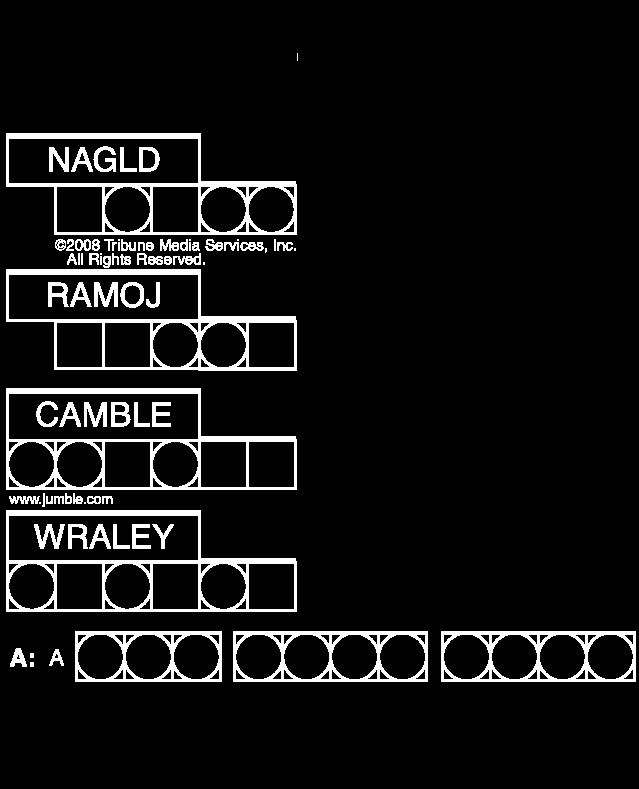
\includegraphics[width=0.4\textwidth]{j1_inverted}
		\caption{Inverted cropped word jumble used for particle analysis}
	\end{figure}


	Before performing particle analysis, the cropped jumble image is inverted. The cropped jumble image is used to reduce the number of noise particles detected.  The resulting inverted image has large square particles in the place of regular letters in a clue entry. Likewise, large circular particles are present in the place of key letters.  When particle analysis is performed on the image it is possible to classify the particles reliably. The area, position, aspect ratio, and solidity of each particle over a threshold area, $a_T$,  are recorded.
	
	$$ a_T = \pi\delta^2 $$
	$$
		\delta = 0.6\bigg(\frac{h_e}{2}\bigg)
	$$
	
	Where $h_e$ is the $y$ distance between the top and bottom of the first answer entry. \par 
	The aspect ratio and solidity of the particles are used to classify them as a regular letter (square particle), a key letter (circular particle), or neither.  A first pass over the particles removes any with an aspect ratio greater than $1.09$.  The particles produced by the clue and answer entries are very regular meaning we can ignore anything even not very significantly non-circular.  After a first pass, each particle remaining in the set is a letter in either an answer entry.  \par 
	To classify each remaining particle, the solidity is examined.  Square particles display a solidity of $1.00$ due to their extreme regularity.  The circular particles display slightly lower solidities ($0.95-0.98$) due to the inability of the computer to perfectly represent the required curve. This rule seems rigid but is surprisingly reliable. \par 
	
	\captionof{table}{Sample particle data from the cropped image shown above. Gray rows are filtered out in the first pass.}
	\begin{center}
		\begin{tabular}{ |c||c|c|c|c|c| } 
			\hline
			Particle ID & Area & X & Y & AR & Solidity \\
			\hline
			\rowcolor[gray]{0.6}
			1&	377794&	364.32&	378.22	&	1.37	&	0.75\\
			\rowcolor[gray]{0.6}
			2&	6864&	102.56&	161.22	&	4.26	&	0.83\\
			3&	2025&	79.5&	209.5	&	1	&	1\\
			4&	1565&	127.45&	209.36	&	1	&	0.97\\
			5&	2025&	175.5	&209.5		&1	&	1\\
			6&	1565&	223.32&	209.5	&	1&		0.97\\
			7	&1565&	271.23	&209.5	&	1	&	0.97\\
			\rowcolor[gray]{0.6}
			8&	6670&	103.35	&297.59	&	4.28	&	0.8\\
			9&	1980&	79.5	&345	&	1.02	&	1\\
			10&	1980&	127.5	&345	&	1.02	&	1\\
			\hline
		\end{tabular}
	\end{center}

	When the classification of each particle is known, it can be combined with the position data to produce an answer template.  By assuming that particles around the same $y$ value belong to the same answer entry, it is possible to determine the position of the key letters within each entry.
	
	\subsubsection{Clue string extraction}
	Clue string extraction is performed to extract the clue strings from the cropped image, and determine their character composition.  To begin, SHLD is re-performed on the cropped image.  This is to ensure no horizontal lines from the comic or other irrelevant parts of the image were detected.  The set of lines rendered by this second application of SHLD is called $L^\prime$. \par \hspace{10pt}
	Viewing the cropped image of the word jumble, it can be seen that each clue string/clue entry pair is bounded by three horizontal lines.  One at the top of the bounding box for the clue string, one at the bottom of the clue entry, and one in-between.  By grouping the lines in $L^\prime$ by threes, then examining the first in each group, it is possible to determine where the top of bounding box for each clue string lies.  By examining the length of the top line in each group, the $x$ position of the end of the clue bounding box can be determined. The location of the bottom of the bounding box can be estimated using $h_e$.  Points just inside in the top left and bottom right corners of the bounding box are easily calculated using an offset\footnote{A static offset was used, but a dynamic offset based on image size could be used if performance of the static offset degraded.}.  These points are then used to extract the clue string from the cropped jumble image.  \par \hspace{10pt}
	Each clue string from a jumble is extracted into its own image file.  Each resulting image file is fed through an OCR system\footnote{pytesseract 0.1.6} to extract the text.  Extracting each individual text region into its own image eases the load on the OCR system and results in high accuracy.
	
	\begin{figure}[H]
		\centering
		\begin{subfigure}{.5\textwidth}
			\centering
			\fbox{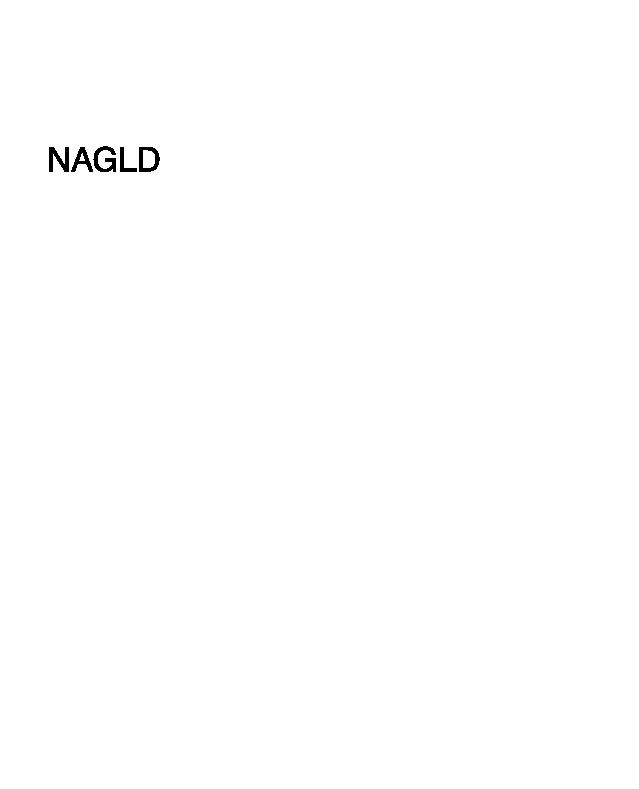
\includegraphics[width=.7\linewidth]{j1_cropped_word0}}
			\label{fig:sub1}
		\end{subfigure}%
		\begin{subfigure}{.5\textwidth}
			\centering
			\fbox{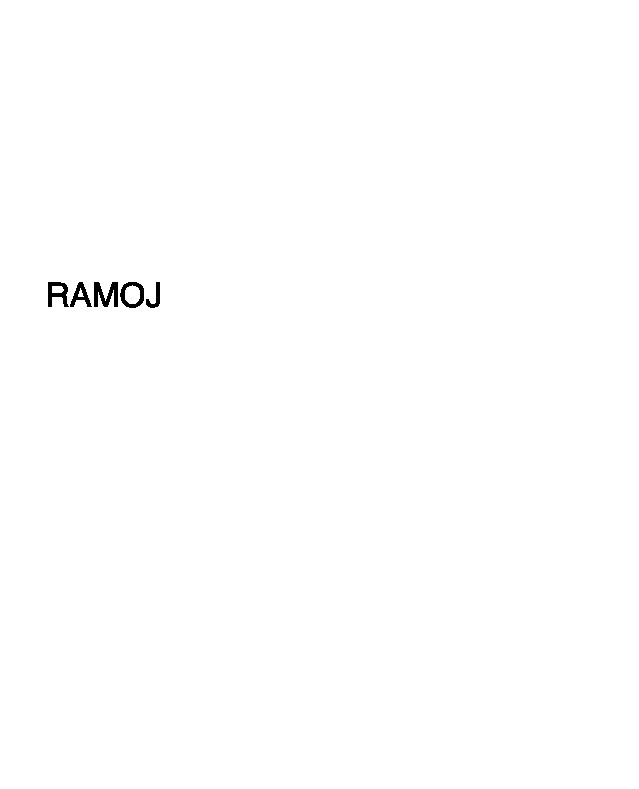
\includegraphics[width=.7\linewidth]{j1_cropped_word1}}
			\label{fig:sub2}
		\end{subfigure}
		\newline 
		\vspace{10pt}
		\begin{subfigure}{.5\textwidth}
			\centering
			\fbox{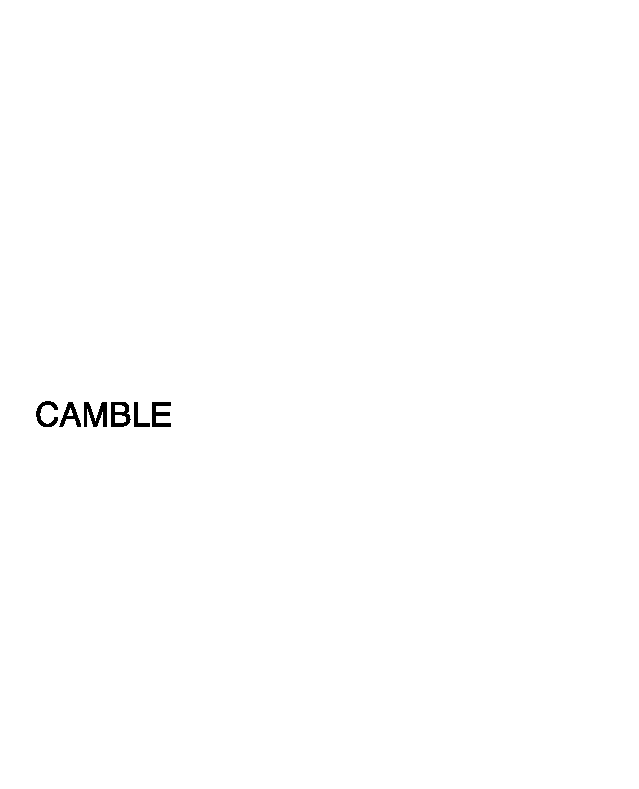
\includegraphics[width=.7\linewidth]{j1_cropped_word2}}
			\label{fig:sub3}
		\end{subfigure}%
		\begin{subfigure}{.5\textwidth}
			\centering
			\fbox{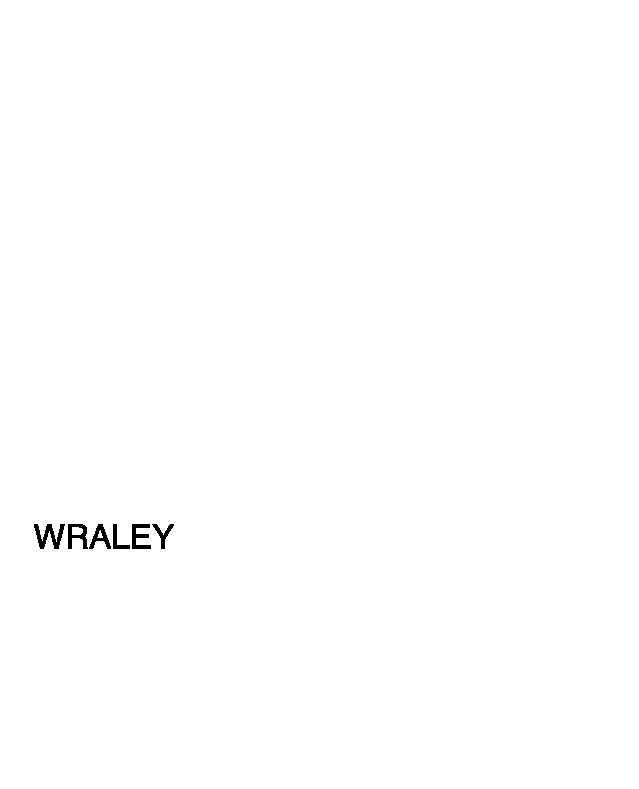
\includegraphics[width=.7\linewidth]{j1_cropped_word3}}
			\label{fig:sub4}
		\end{subfigure}
		\caption{Words extracted from the cropped jumble.}
	\end{figure}

	\subsection{Solving}
	Using the information gained from the particle analysis and clue string extraction subprocesses, an attempt is made to solve the word jumble.  \par 
	
	\subsubsection{Solving the clue anagrams}
	The first solving sub-step involves the solving of the clue anagrams.  This is done by brute force comparison against a dictionary of around $100,000$ of the most popular English words. While a seemingly large problem, the solving of all clue anagrams is one of the most least time intensive sub-steps involved in finding the solution to the final anagram. \par\hspace{10pt}
	 To solve each clue, comparisons are done between the sorted version of each clue anagram and a sorted version of each word in the dictionary file.  If the sorted strings match, then the word is a possible solution to the anagram.  Most clues found in word jumbles only have one possible solution, however approximately $20\%$ have more than one, sometimes with up to three. \par 
	 
	 \subsubsection{Extraction of the final anagram}
	 Using the knowledge gained through particle analysis and the solutions above, the key letters in each clue anagram solution can be found.  The key letters from each clue anagram solution form a string that is the final anagram.  The final anagram represents the final challenge of the puzzle.
	 
	\subsubsection{Final answer format deduction}
	 The final answer to a word jumble is often a phrase spread across two or more words.  To aid the solving of the final anagram we must know how many words are in the final answer, and the length of each word. To determine these key quantities, $L^\prime$ is used. \par \hspace{10pt}
	 Through $C_{ans}$ it is guaranteed that the last horizontal line in $L^\prime$ is part of the bottom bounds for the final answer entry.  By noting the $y$ height of the last element in $L^\prime$ a baseline for the height of the bottom of the answer is gained.  $L^\prime$ is then reversed and iterated over, at the same time counting the number of lines at the noted $y$ height.  The number of lines at the height gives the number of words in the answer. The length of each of these lines is also noted.  Using the lengths of each line, and the total string length of the final anagram, the phrase structure of the final solution can be deduced. 

	 \subsubsection{Final anagram solving}
	 The final anagram is solved by brute force comparison. The process starts with the generation of all possible permutations of the anagram.  Each permutation is then partitioned to match the word format of the final answer.  Each partition of the permutation is then compared against a dictionary to determine its validity as a word.  If all partitions of the permutation are words, then the phrase is a possible solution to the final anagram.\par\hspace{10pt}
	 This method of solving is inefficient due to the large possible number of permutations of the final anagram.  Some final anagrams are up to thirteen characters in length, this leads to upwards of six billion possible permutations.  An attempt to optimize the brute force approach is made, but nonetheless, the method only proves usable for final anagrams under twelve characters in length. \par \hspace{10pt}
	 The optimizations to the brute force comparison method are made through a specialized dictionary structure, and a permutation cache.
	 
	 \paragraph{Dictionary structure}
	 The dictionary structure used in solving the final anagram is queried thousands of times per second, thus lookups in the structure must be efficient to ensure a reasonable solution time. The dictionary consists of a series of nested hash tables.  In the first layer the keys represent the first letter of a word, and each key points to another hash table.  The keys of the second layer of hash tables are integers representing the length of the strings.  Each integer key points to a final hash table which uses the word as a key.  The word key points to a true value, signaling the word is valid.  If an entry for the word is not found in the final layer of hash table, then it is assumed the word is not valid.
	 
	 \paragraph{Permutation cache}
	 Of the possibly billions of permutations generated from the final anagram, usually not all are unique.  Logically it makes sense to remove the duplicate permutations before iterating over them to determine their validity as a solution.  However, memory constraints make this unfeasibly scalable.  To get around this problem a hash table representing a cache of previously seen permutation strings is maintained. Every permutation string is added to this hash table as it is seen. The hash table is limited to $10,000,000$ items (roughly 1GB of memory).  The table randomly removes an item when it is full and requires room for a new item.\par 
	 
	 \vspace{10pt}
	 
	 In practice, the permutation cache is used to check if a permutation string has been seen before deciding to partition it, and validate it against the dictionary.  Obviously this is not perfectly reliable, however it is a fair solution considering the memory overheads required for greater caching.  Together with the fast lookup dictionary, the system is able to check roughly $100,000$ solutions every second.
	 
	\section{Results} 
	Overall, the algorithm provided above does a reasonable job of solving word jumbles, and provided good feature extraction from the puzzle. \par \hspace{10pt}
	The algorithm was tested on 10 word jumble images of various quality ranging in size from 350px to 2000px tall.\par 
	
	\subsection{Clue segmentation and recognition}
	The methods used to segment the clue text from the cropped word jumble image result in a series of images with no features besides the characters of a single word.  This makes it very easy for the OCR system used to recognize the characters.  The algorithm is able to extract and completely resolve all clues from all images in the test set for an accuracy of 100\%.
	
	\subsection{Clue solving}
	100\% of the clues extracted from the cropped images can be unscrambled to one or more English words.  Most clues resolve to a single unique word, however some have multiple matches.  In the case of multiple matches, a lazy approach is taken and the first match is used. 
	
	\subsection{Final anagram extraction}
	The 10 images in the test set yielded 40 unique anagram clues (excluding final anagrams).  Each clue corresponded to an answer entry with one or more key letters.  Solidity and aspect ratio based particle analysis was successful in identifying all key letters in the answer entry for 92.5\% (37/40) of the clues. No false positives were detected in the clues which had all key letters identified. The count of key letters in each clue entry as determined by the algorithm was within one of the actual count for 100\% of the clue entries sampled.
	
	\subsection{Answer format deduction}
	In the algorithm, the phrase structure of the final answer was determined by examining the horizontal lines closest to the bottom of the cropped image in combination with the length of the final anagram. 
	This proves a very accurate method, as it is able to deduce the number of words in the final answer, and the length of each word for 90\% (9/10) of the test images\footnote{j7.png is the only file that it does not work for.}.
	
	\subsection{Final anagram solution}
	While each individual piece needed for a successful solving system is in place, the combination of the elements into a contiguous solution is more difficult.  Each piece of the algorithm relies on the previous, thus a fracture in any component means the resolution of a final anagram solution is nearly impossible.  \par \hspace{10pt}
	The major challenge in finding a final anagram solution is computation time.  Long final anagrams can take days to resolve using the optimized brute force method described previously. \par \hspace{10pt}
	Even when the solution is easily computationally reachable using the optimized brute force, it is likely that multiple possible solutions exist.  Some images in the test set produce over 2000 possible solutions. \par
	 
	 \captionof{table}{Number of possible solutions for the final anagram. - denotes the size could not be computed in realistic time. N/A means some error occured before final anagram solving.}
	 \begin{center}
	 	\begin{tabular}{ |c||c| } 
	 		\hline
	 		Image & Possible solutions found \\
	 		\hline
	 		$j1.png$ & 2244 \\
	 		$j2.png$ & -\\
	 		$j3.png$ & 1 \\
	 		$j4.png$ & 18 \\
	 		$j5.png$ & 466 \\
	 		$j6.png$ & - \\
	 		$j7.png$ & N/A (Improper answer format deduced.) \\
	 		$j8.png$ & N/A (Key letter location mistakes occur.) \\
	 		$j9.png$ & 2 \\
	 		$j10.png$ & 112 \\
	 		\hline 	
	 	\end{tabular}
	 \end{center}
 
	That said, it is possible for the algorithm to significantly decrease the size of the solution space\footnote{Size of the solution space is calculated as the number of permutations of a string of the same length as the final anagram multiplied by $0.65$ (to represent an estimate of 35\% repeated permutations).} for the final anagram in 60\% (6/10) of the test images.  \par 
	
	\begin{figure}[h]
		\centering
		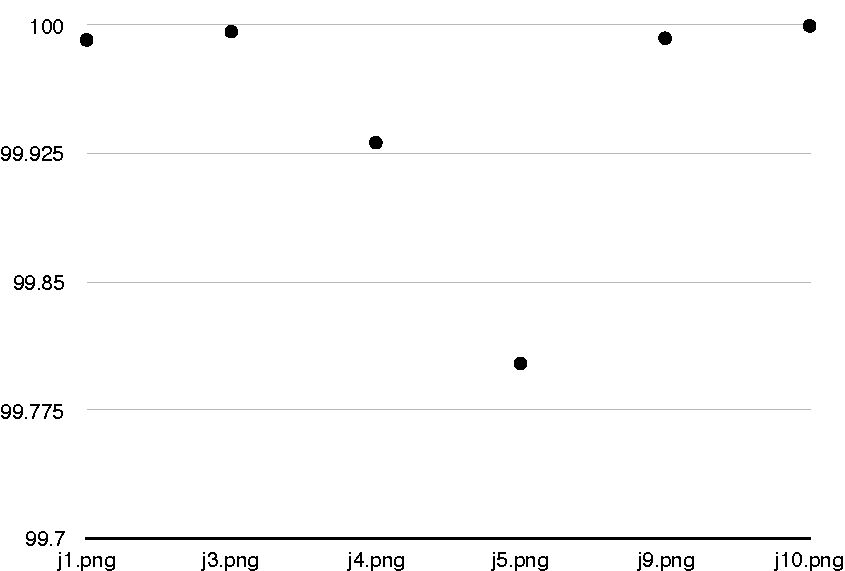
\includegraphics[width=.85\textwidth]{graph}
		\caption{Percent reduction in solution space size through application of the algorithm.}
	\end{figure}

	Of the eight images that did not encounter errors before the final anagram solving, only six were solvable in reasonable time.  Two images\footnote{$j2.png$ and $j6.png$} contained final anagrams over twelve characters in length, taking an unreasonable amount of time to solve even using an optimized brute force method.  Nonetheless, the six images that saw a substantial reduction in solution space size were solved in very reasonable time.
	
	\begin{figure}[h]
		\centering
		\includegraphics[width=.85\textwidth]{time}
		\caption{Time required to narrow final anagram solution space.}
	\end{figure}
	
	\section{Discussion}
	While in general the algorithm provides a decent solution to the problem, improvements can be made.  \par \hspace{10pt}
	The core technique employed to landmark and extract most features is SHLD.  For most word jumbles this works extremely well, however this technique fails miserably on images that have been rotated or contain a large amount of noise. \par\hspace{10pt}
	To improve the solving of the individual clue anagrams, a word popularity index could be employed to determine the most likely word when the clue can be unscrambled to more than one possible word. In the same vein, a more "intelligent" system could be used to find appropriate permutations of the final anagram. \par \hspace{10pt}
	The final anagram extraction could also be improved.  By employing a segmentation based strategy on the pre-filtered particles, rather than using a static bound when examining solidity, better classification could be achieved.  The circular and square particles always display different solidities as noted above.  However, the static bound that is currently used to determine the classification of the particle can be unreliable in rare cases. To combat this particles could be grouped based on like solidities rather than partitioned using the static bound. \par \hspace{10pt}
	Errors in the answer format deduction are more common in lower quality, small images.  This is a pitfall of the current SHLD implementation.  In future, an implementation which joins together line segments separated in the $x$ by a small gap may help solve this problem.  For now, the issue is pertinent to only a small fraction of the dataset, so it is accepted.\par \hspace{10pt}
	To improve the solution speed and memory footprint, a probabilistic data structure such as a bloom filter could be used in place of a hash table for the permutation cache.  The solving of long final anagrams slows significantly after the cache becomes full and must start randomly removing an element to add each new permutation string.  A bloom filter may help to store more items in the cache while maintaining a memory footprint comparable to the allocations currently used. \par 
	
	\section{Conclusion}
	Overall, the algorithm presented provides near perfect extraction and solving of clues from a large majority of word jumbles.  Additionally, success is also found in drastically narrowing the solution space of the final anagram, and in some cases providing a definite solution.

	
	
	
\end{document}